\chapter{Beyond Solid-On-Solid : the Particles-Over-Particles model}

In fact, if the height profiles represent particle numbers, if we fix the total number of particles to be $N$ and take them to be identical the partition function is given by
\begin{equation}
    Z_N = \frac{1}{N!}\sum_{h_1,h_2\cdots h_L} \delta_{\sum_{i=1}^L h_i, N}\frac{N!}{\prod_{i=1}^L h_i!} \exp\left(-\beta \sigma \sum_{i=1}^L |h_{i+1}-h_i| -\beta\sum_{i=1}^L V(h_i)\right).
\end{equation}
Here the combinatorial term $\frac{N!}{\prod_{i=1}^L h_i!}$ represents the number of ways that the $h_i$ particles on each site can be chosen from the $N$ particles available. The constraint on the particle number makes the computation of the partition function at fixed $N$ complicated both analytically and numerically. However if we change to the grand canonical ensemble using
the formula
\begin{equation}
    \Theta = \sum_{N} \exp(\beta\mu N) Z_N,
\end{equation}
where $\Theta$ is the grand partition function and $\mu$ the chemical potential, we find
\begin{equation}
    \Theta = \sum_{h_1,h_2\cdots h_L} \frac{1}{\prod_{i=1}^L h_i!} \exp\left(-\beta \sigma \sum_{i=1}^L |h_{i+1}-h_i| -\beta\sum_{i=1}^L[ V(h_i)-\mu h_i]\right).
\end{equation}
The grand partition function can then be written as 
\begin{equation}
    \Theta = \sum_{h_1,h_2\cdots h_L} \exp\left(-\beta H_{eff}(h_1,h_2\cdots h_L)\right)
\end{equation}
where 
\begin{equation}
    H_{eff}= \sigma \sum_{i=1}^L |h_{i+1}-h_i| +\sum_{i=1}^L [V(h_i)-\mu h_i +\frac{1}{\beta}\ln(h_i !)].
\end{equation}

\begin{figure}
    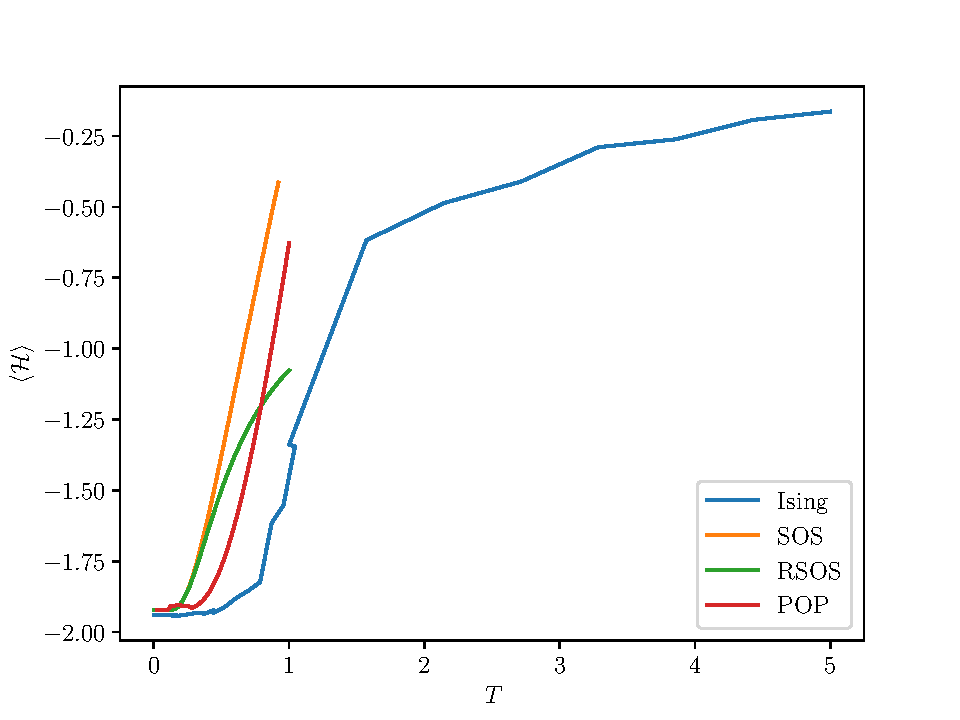
\includegraphics{pop/comparaison-modeles.pdf}
\end{figure}
\begin{figure}
    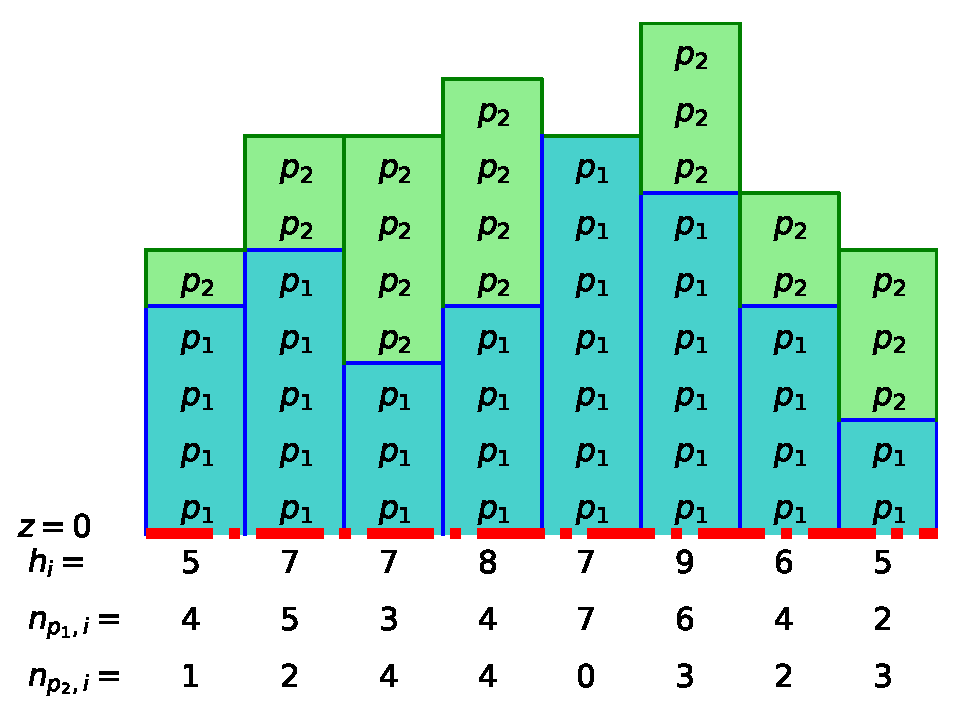
\includegraphics{pop/figure-pop.pdf}
\end{figure}